% 1. Presentación del problema de infiltración de agua
% 1.1 Ventajas de la simulación % Arley ayuda, sin tantas ecuaciones.
% Optimizar el uso del agua en el suelo, lograr el mayor contacto entre las capas periféricas de la raíz del suelo. 1 gota de aceite contamina un litro de agua. riego por surco, problema del percolación, los nutrientes son llevados, ejemplo con el café tradicional. problema
% cantidad desmedida de agua porque el suelo pierde sus nutrientes, %60% de eficiencia
% ejemplo de la caña: pesticidas, exceso de agua, etc (ciclo).
% el perder agua es mucho más caro para la humanidad.
% aportar a la agricultura de precisión
% ruta apoplástica (explica la interacción de la raíz agua)
% % el efecto de las algas (dia/noche) se puede explicar con el cloropasto () y la mitocondria (respiración)
% qué solución hay.
% de lo general a particular.
% [1] Ref.
\section{Presentation of water infiltration problem}
\subsection{Importancia}
\subsection{Justificación}
\subsection{Descripción del problema}
\subsection{Ecological footprint of the water cycle on agriculture}

\begin{frame}
	\frametitle{\subsecname}
	\begin{figure}[ht!]
		\centering
		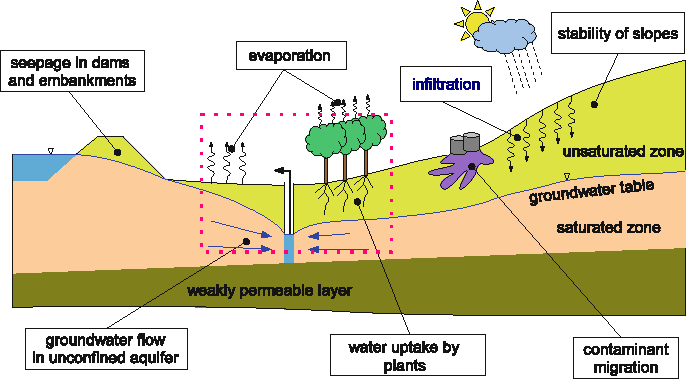
\includegraphics[height=7cm]{contamination}
	\end{figure}
	\note{
		En la diapositiva se muestra una de estas situaciones diarias.

		También se tiene un anexo donde se estudia un software libre
		como es \lstinline|wxmaxima|.
	}
\end{frame}
% TODO: Poner la imagen en el centro, y en ovalos redondeados colocar las ideas del primer p'arrafo
% TODO: es decir, crecimiento poblacional, demanda de alimentos
% TODO: Agricultura que no es de precision, agua.
% https://tex.stackexchange.com/questions/96289/how-to-connect-beamer-blocks-by-arrows
\subsection{Problem}
\begin{frame}
	\frametitle{\subsecname}
	\begin{minipage}{0.6\textwidth}
		\begin{itemize}
			\item

			      Urban planning, together with population growth
			      over the years, so food demand increased and exploit more natural resources for agricultural activities,
			      however eagerness to meet this demand we have neglected the good management of natural resources and the stability
			      of the surrounding ecosystems. \cite{Latham1997}
			      % El desarrollo urbano, en conjunto con el crecimiento poblacional
			      % a lo largo de los años, ha llevado al alza de la demanda de
			      % alimentos por parte del ser humano, motivo por el cual se se a
			      % visto en la obligación explotar cada vez más los recursos naturales que lo rodean y utilizar más terrenos para diversas actividades agrarias, sin embargo en su afán de suplir dicha demanda ha descuidado el buen manejo de los recursos naturales y la estabilidad de los ecosistemas que lo rodean.

			\item

			      Currently in agriculture, one of the most frequent problems with the greatest environmental impact generated by poor crop management is the inefficient use of water resources, by implementing inefficient irrigation systems when trying to meet the water demand generated by plants. It is also one of the most important points addressed in environmental issues and is not only of concern because of the waste of water but also because of the damage and losses that can be caused in the physicochemical properties of the soil.

			      % Actualmente en la agricultura uno de los problemas más frecuentes  y de mayor impacto ambiental que genera el mal manejo de los cultivos, es el uso ineficiente de los recursos hídricos, al implementar sistemas de riego poco eficaces, al tratar satisfacer la demanda hídrica que generan las plantas. Además es uno de los puntos más importantes que se abordan en temas ambientales y que no solo preocupa por el desperdicio de agua sino también por el daño y las pérdidas que puede ocasionar en las propiedades fisicoquímicas del suelo.
			      % https://proain.com/blogs/notas-tecnicas/calidad-del-agua-para-riego-agricola
		\end{itemize}
	\end{minipage}
	\begin{minipage}{0.37\textwidth}
		\begin{figure}[ht!]
			\centering
			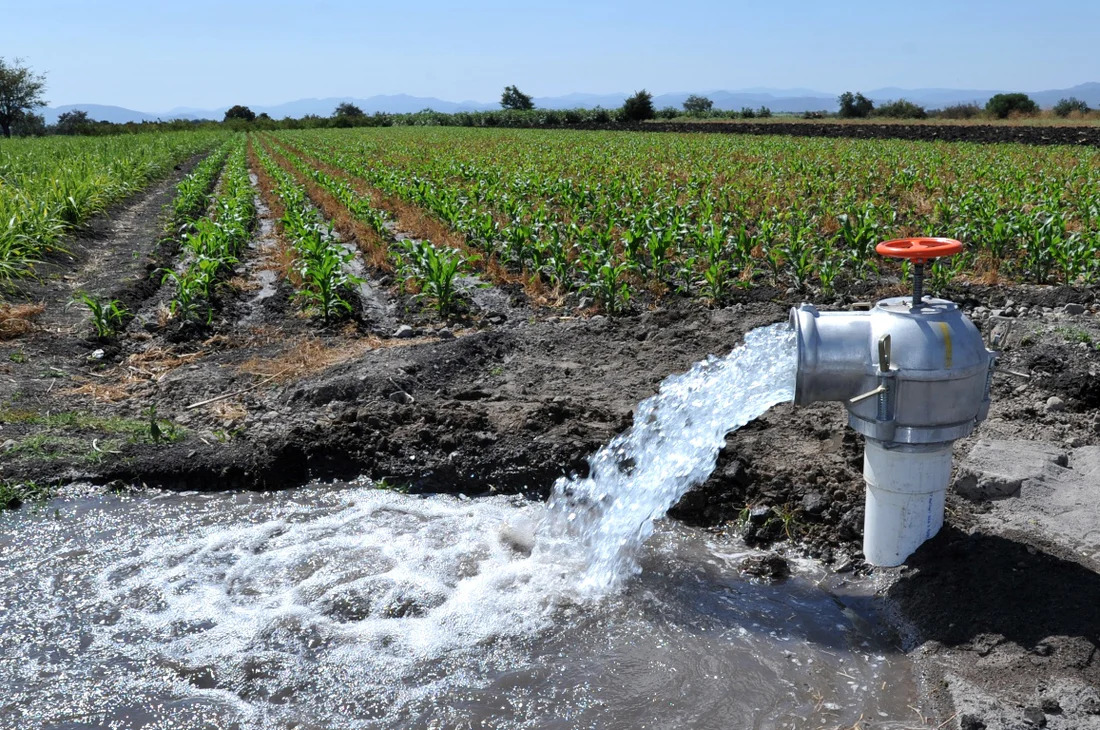
\includegraphics[height=4cm]{wasted_water}
		\end{figure}
	\end{minipage}
\end{frame}

\begin{frame}
	\frametitle{\secname}
	\begin{minipage}{0.5\textwidth}
		\begin{itemize}
			\item .
		\end{itemize}
	\end{minipage}
	\begin{minipage}{0.47\textwidth}
		\begin{figure}[ht!]
			\centering
			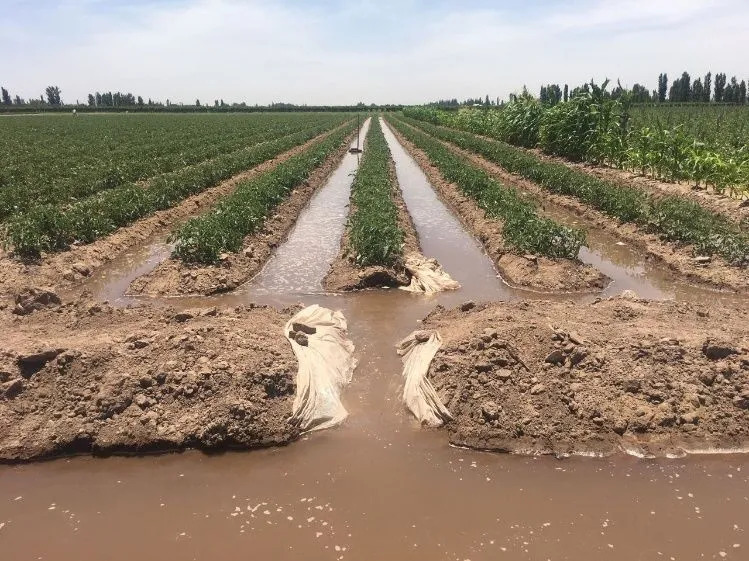
\includegraphics[height=5.5cm]{water_waster2}
			% https://www.agromeat.com/284499/conceptos-tecnicas-y-estrategias-en-uso-eficiente-del-agua-de-riego
		\end{figure}
	\end{minipage}
\end{frame}
% Irricad

\begin{frame}
	\begin{center}\Huge % TODO: Poner sobre un fondo con relleno sin bordes.
		What is the capillarity water soil?
	\end{center}
\end{frame}

\subsection{Capillarity}

\begin{frame}
	\frametitle{\subsecname}
	\begin{minipage}{0.5\textwidth}
		\begin{align*}
			\Delta p=p_{\mathrm{a}}-p_{\mathrm{w}} & =
			\sigma_{\mathrm{aw}}\left(\frac{1}{r_{\mathrm{c} 1}}+\frac{1}{r_{\mathrm{c} 2}}\right)
			=\frac{2 \sigma_{\mathrm{aw}} \cos \psi}{r_{\mathrm{c}}}                                  \\[\baselineskip]
			\sigma_{\mathrm{aw}}\cos\psi           & =\sigma_{\mathrm{Sa}}-\sigma_{\mathrm{Sw}},\quad
			h_{\mathrm{c}} =\frac{1.5 \times 10^{-5}}{r_{\mathrm{c}}}
		\end{align*}
		\begin{itemize}
			\item $\sigma_{\mathrm{aw}}$ is the surface tension of the air-water interface.
			\item $\sigma_{\mathrm{Sa}}$ is the surface tension of the solid-air interface.
			\item $\sigma_{\mathrm{Sw}}$ is the surface tension of the solid-water interface.
			\item $\psi$ is the wetting angle.
		\end{itemize}
	\end{minipage}
	\begin{minipage}{0.47\textwidth}
		\begin{figure}[ht!]
			\centering
			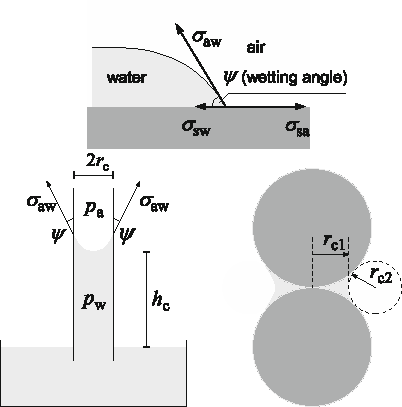
\includegraphics[height=6.2cm]{capillar_preassure}
		\end{figure}
	\end{minipage}
\end{frame}

\subsection{Soil water content} % Humedad en el suelo
\begin{frame}
	\frametitle{\subsecname}
	\begin{figure}[ht!]
		\centering
		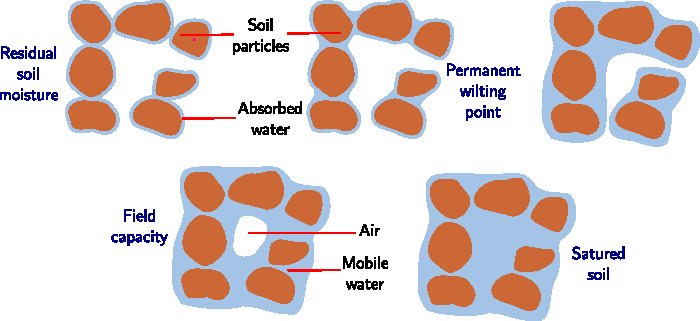
\includegraphics[height=6.8cm]{wetness}
	\end{figure}
\end{frame}